\documentclass[
	handout,
%  	aspectratio=43
  	aspectratio=169
]{beamer}

\usepackage[utf8]{inputenc}
\usepackage[german]{babel}
\usepackage[figurename=Bild]{caption}
\usepackage{graphicx}
\usepackage{amsmath}
\usepackage{scrextend}
\usepackage{xcolor,colortbl}	
\usepackage{lmodern}	
\usepackage{amsmath,amssymb}
\usepackage{booktabs}

\title[Semesterprojekt KNIME]{Data Mining}

\date{18.06.2021}
\author[C. Werner, J. Prothmann]{C. Werner, J. Prothmann}


\institute{Bereich Elektrotechnik und Informatik}
\usetheme{Wismar}	% Design der Hochschule Wismar
\usecolortheme{FIW}

% Die Navigationshilfen unteren Folienrand kann man ausblenden
\beamertemplatenavigationsymbolsempty
% \beamertemplatefootempty

% Wenn mathematische Umgebungen in klassischer "Mathe-Schrift"
% dargestellt werden sollen, folgende Zeile entkommentieren.
%\usefonttheme[onlymath]{serif}

% Zeige Abschnittstitel auf separater Folie vor jedem Abschnitt
%\AtBeginSection{\frame{\sectionpage}}

\begin{document}
	\begin{frame}[plain]
		\titlepage
	\end{frame}

	\begin{frame}[allowframebreaks]{Gliederung}
		\tableofcontents
	\end{frame}
		
	\section{Entscheidungsbäume}
	
		\begin{frame}{Decision Tree Learner}
			\begin{itemize}
				\item Standardknoten von Knime
				\item Zielattribut: nominal
				\item Entscheidungsfindungsattribute: nominal, numerisch
				\item Qualitätsmaße für Splitberechnung:
				\begin{itemize}
					\item Gini-Index
					\item Gain-Ratio
				\end{itemize}
				\item Pruning möglich
			\end{itemize}
		\end{frame}

		\begin{frame}{SimpleCart}	
			\begin{itemize}
				\item Weka-Knoten
				\item Erzeugung von Binärbäumen
				\item Pruning möglich
				\item Je höher der Informationsgehalt eines Attributs in Bezug auf die Zielgröße, desto weiter oben im Baum findet
sich dieses Attribut. 
			\end{itemize}
			\begin{center}
				\begin{figure}[h]
					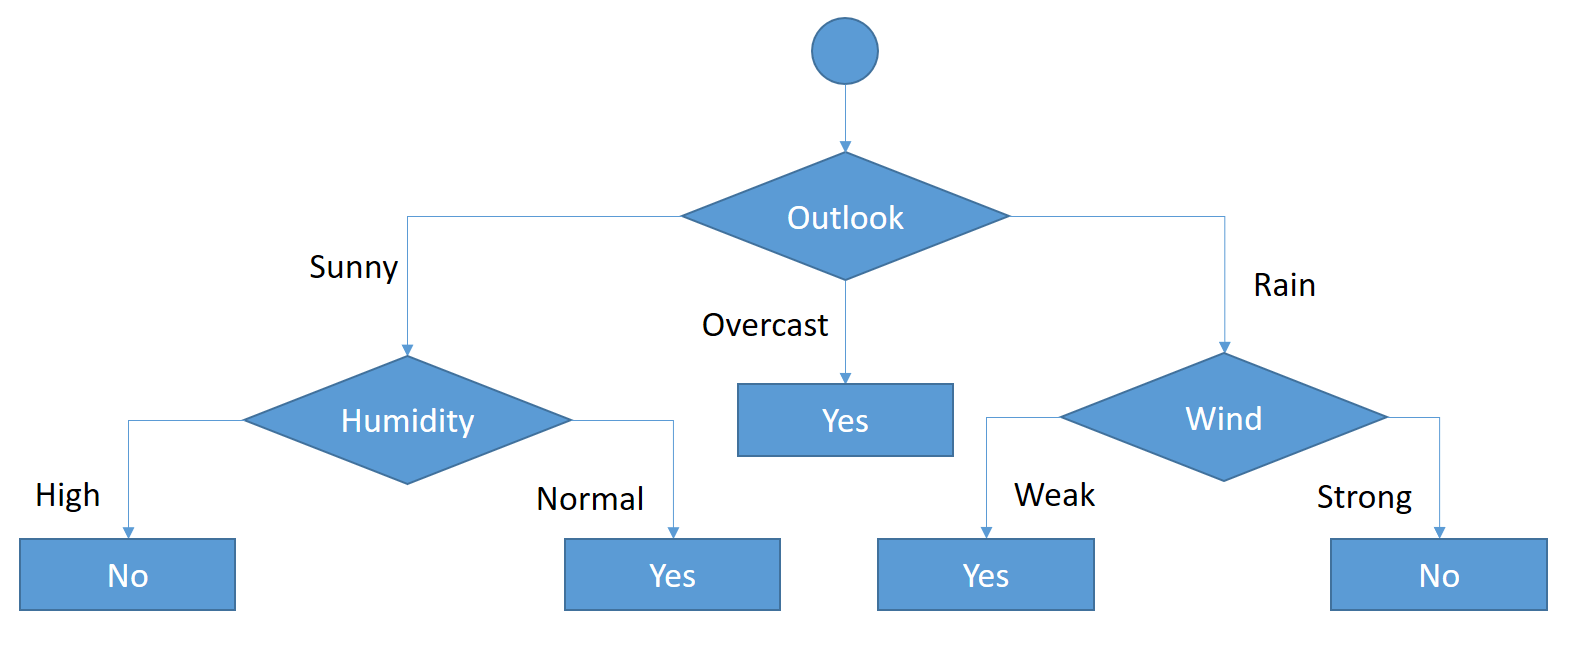
\includegraphics[scale=0.2]{../pictures/cart-tree.png}
					\caption{CART Tree Beispiel}		
				\end{figure}		
			\end{center}
		\end{frame}

		\begin{frame}{J48}		
			\begin{itemize}
				\item Weka-Knoten
				\item C4.5 Algorithmus von J. Ross Quinlan
				\item Ähnlich zu CART, jedoch kein Binärbaum
				\item Deutlich breiter und weniger tief als CART
				\item Pruning möglich
			\end{itemize}
		\end{frame}

		\begin{frame}{NBTree}
			\begin{itemize}
				\item Weka-Knoten
				\item Hybridalgorithmus aus Entscheidungsbaum- und Naive-Bayes-Klassifikatoren
				\item \glqq{}klassische\grqq{} Knoten
				\item Blätter enthalten Naive-Bayes’sche Klassifikatoren
			\end{itemize}	
			
			\begin{center}
				\begin{figure}[h]
					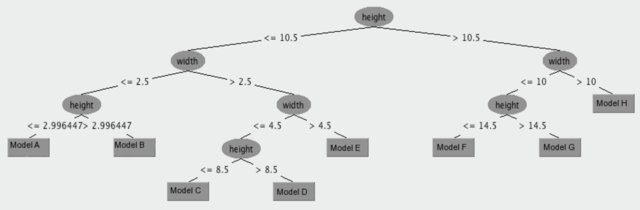
\includegraphics[scale=1]{../pictures/NBTree-classifying-MAC-Felinae.jpg}
					\caption{NB Tree Beispiel}		
				\end{figure}		
			\end{center}
			
			
		\end{frame}

		\begin{frame}{REPTree}		
		\end{frame}

		\begin{frame}{LMT}		
		\end{frame}

		\begin{frame}{DecisionStump}		
		\end{frame}

		\begin{frame}{J48Graft}		
		\end{frame}

		\begin{frame}{BFTree}		
		\end{frame}

		\begin{frame}{RandomTree}		
		\end{frame}

		\begin{frame}{RandomForest}		
		\end{frame}

		\begin{frame}{FT}		
		\end{frame}





	\begin{frame}{Test}
		\begin{columns}[T]
   				\begin{column}{.5\textwidth}
					\begin{itemize}
						\item mehr Energie und Sorgfalt bei Suchanfragenformulierung
						\item Wahl der passenden Suchbegriffe
						\item Nutzung spezieller Befehle und Operatoren
						\item \glqq{}Effective internet searching is part science, part art, part skill and part luck.\grqq{} (Bradley 2013, S.18)
					\end{itemize}
    				\end{column}
    				
    				\begin{column}{.5\textwidth}
					\begin{figure}[h]
						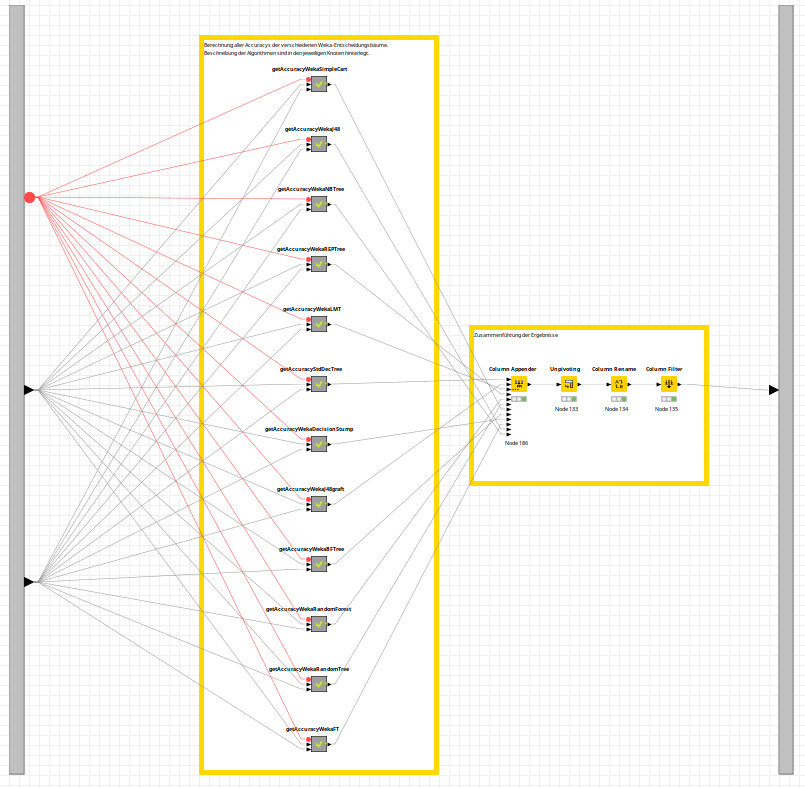
\includegraphics[scale=0.2]{../pictures/trees-workflow-getAccuracys.png}
						\caption{Bewertbarkeit des Sucherfolgs nach Anfragetyp (Lewandowski 2018, S.216)}		
					\end{figure}					
    				\end{column}
  			\end{columns}
	\end{frame}

\end{document}
